% Provenance (never printed): see sources/outline_sources.md (Year 3:
% Darcy's law; permeability; aquifer types; the groundwater-flow equation;
% pumping tests; solute transport, in principle).
% Brief: sources/book5/BRIEFS.md, ch. 23. Curves from figdata/bachelor-3/
% theis.py, flow_net.py and advection_dispersion.py; the site of Varden-3 from
% figdata/shared/region.py (read only). Exercise and problem values in the
% Book 5 scratch calculator calc/ch23.py. The wells, the dam, the tests and
% the solutes are invented.
\chapter{जलभूविज्ञान}\label{ch:b3:hydrogeology}

एक नया कुआँ प्रतिदिन \qty{2160}{m^3} पानी एक चूना-पत्थर से निकालता है, जो
एक फ़ार्म के नीचे कुछ सौ मीटर गहराई पर है। शुरू में फ़ार्म के अपने कुएँ पर कोई असर नहीं पड़ता।
एक महीने बाद उसका पानी लगभग \qty{2}{m} नीचे आ जाता है, यद्यपि
वह एक किलोमीटर दूर है और पंपिंग स्टेशन ने उससे कभी एक बूँद नहीं खींची। नए कुएँ के
चारों ओर का जल-स्तर समान रूप से नहीं गिरा है: वह एक
शंकु में धँस गया है, और यह शंकु तेज़ी से उस चट्टान में फैला है जिसमें पानी
स्वयं प्रतिदिन कुछ सेंटीमीटर चलता है। यह अध्याय वह भौतिकी विकसित करता है जो
दोनों संख्याओं का पूर्वानुमान करती है: दाब का तीव्र प्रसार और
पानी की धीमी यात्रा, 1856 में मिले एक अनुभवजन्य नियम से।
% ledger: heath:darcy

\begin{recall}
सरंध्रता, पारगम्यता, भौम जलस्तर, भूजल, जलभृत, सोते
और कुएँ विद्यालय की पुस्तकों में हैं, साथ में पानी का निवास काल और
जीवाश्म भूजल। श्यानता, नली में बहाव के लिए पॉइज़्यूई का नियम
और विसरण समीकरण भौतिकी की पुस्तकों में हैं। त्रुटि फलन
और उसका उपयोग करने वाले विसरण समीकरण के हल
अध्याय~\ref{ch:b3:lithosphere-thermal-models} में हैं। वार्डन पहाड़ियाँ, श्रृंखला का काल्पनिक क्षेत्र,
अपने बलुआ पत्थर, चूना-पत्थर, शेल और चॉक के साथ,
विद्यालय की पुस्तकों से अभ्यासों का क्षेत्र है।
\end{recall}

\section{शीर्ष और डार्सी का नियम}\label{sec:b3:hydrogeology:darcy}

भूमिगत पानी उस स्थान से चलता है जहाँ उसकी इकाई भार की यांत्रिक ऊर्जा अधिक है,
उस स्थान की ओर जहाँ वह कम है। चूँकि यह धीरे चलता है, इसकी गतिज ऊर्जा नगण्य है,
और यह ऊर्जा दो भागों में होती है: पानी की ऊँचाई और उसका
दाब।

\begin{definition}[जलीय शीर्ष; जलीय प्रवणता]\label{def:b3:hydrogeology:head}
संतृप्त भूमि के किसी बिंदु का \emph{जलीय शीर्ष}\index{जलीय शीर्ष}
होता है
\[
h = z + \frac{p}{\rho g} ,
\]
यह योग है: किसी बिंदु का एक संदर्भ तल के ऊपर का \emph{उन्नतांश शीर्ष} $z$ और
\emph{दाब शीर्ष} $p/(\rho g)$ है, जहाँ $p$ वायुमंडलीय दाब से ऊपर पानी का दाब है।
यह वह ऊँचाई है जहाँ तक पानी एक नली में चढ़ता है,
पीज़ोमीटर, जो केवल उसी बिंदु पर खुली है। \emph{जलीय
प्रवणता}\index{जलीय प्रवणता} $\nabla h$ है; प्रवाह के अनुदिश दो बिंदुओं के बीच,
जो $L$ दूरी पर हैं, इसका परिमाण $\Delta h/L$ है।
\end{definition}

\begin{omfigure}
\centering
\begin{tikzpicture}[>=stealth, font=\small, x=1cm, y=1cm]
\fill[omLithAlluv!60] (0,-0.6) rectangle (7,3.2);
\fill[omSea!45] (0,-0.6) rectangle (7,1.9);
\draw[thick, brown!60!black] (0,3.2) -- (7,3.2);
\draw[omDef, dashed] (0,1.9) -- (7,1.9);
\node[omDef, font=\scriptsize, anchor=south east] at (6.9,1.92) {भौम जलस्तर};
% piezometer
\fill[white] (3.3,0.4) rectangle (3.7,4.0);
\draw[thick] (3.3,0.7) -- (3.3,4.0); \draw[thick] (3.7,0.7) -- (3.7,4.0);
\draw[thick, densely dotted] (3.3,0.4) -- (3.3,0.7); \draw[thick, densely dotted] (3.7,0.4) -- (3.7,0.7);
\fill[omSea!70] (3.32,0.4) rectangle (3.68,2.6);
\draw[omDef, thick] (3.3,2.6) -- (3.7,2.6);
\fill (3.5,0.55) circle (0.06);
\node[font=\scriptsize, anchor=west] at (3.75,0.55) {छलनी, बिंदु $P$ पर};
% datum
\draw[black!60] (0,-0.6) -- (7,-0.6);
\node[font=\scriptsize, anchor=north west] at (0,-0.62) {संदर्भ तल, $z = 0$};
% heads, on the left of the tube
\draw[<->] (2.5,-0.6) -- node[left, font=\scriptsize] {$z$} (2.5,0.55);
\draw[<->] (2.5,0.55) -- node[left, font=\scriptsize] {$p/\rho g$} (2.5,2.6);
\draw[black!40, densely dashed] (2.4,0.55) -- (3.3,0.55);
\draw[black!40, densely dashed] (1.0,2.6) -- (3.3,2.6);
\draw[<->, thick, omThm] (1.1,-0.6) -- node[left, font=\scriptsize] {$h$} (1.1,2.6);
\node[font=\scriptsize, anchor=south] at (3.5,4.0) {पीज़ोमीटर};
\end{tikzpicture}

\par\smallskip{\small पीज़ोमीटर, एक नली जो केवल अपनी छलनी पर खुली है। पानी
उसमें बिंदु $P$ के \omterm{def:b3:hydrogeology:head}{जलीय शीर्ष} पर खड़ा होता है: उसका उन्नतांश $z$ और
उसका दाब शीर्ष। यहाँ नली में स्तर भौम जलस्तर से ऊपर है,
जैसा उस स्थिति में होता है जहाँ पानी किसी सोते की ओर
या नदी की ओर ऊपर चढ़ता है।}\label{fig:b3:hydrogeology:head}
\end{omfigure}

1856 में फ़्रांसीसी इंजीनियर हेनरी डार्सी ने पानी के प्रवाह को
रेत के स्तंभों से होकर मापा और पाया कि वह प्रति इकाई लंबाई
शीर्ष-ह्रास के समानुपाती है। प्रवाह धारावाही है: पानी अलग-अलग धारारेखाओं का अनुसरण करता है।
% ledger: heath:darcy

\begin{theorem}[डार्सी का नियम]\label{thm:b3:hydrogeology:darcy}
संतृप्त सरंध्र माध्यम में प्रति इकाई समय में प्रति इकाई क्षेत्रफल से गुज़रने वाला
पानी का आयतन है
\[
\vec q = -K\,\nabla h ,
\]
जहाँ $K$ माध्यम और तरल पर निर्भर करता है। ऐसे माध्यम में जिसके रंध्र
त्रिज्या $a$ की समानांतर सीधी नलियाँ हैं, जो आयतन का अंश $n$ घेरती हैं,
तब पॉइज़्यूई का नियम इस नियम को इस रूप में देता है
\[
K = \frac{k\rho g}{\mu}, \qquad k = \frac{na^2}{8} ,
\]
जहाँ $\mu$ पानी की श्यानता है।
\end{theorem}
\index{डार्सी का नियम}

\begin{proof}
पहला कथन डार्सी का अनुभवजन्य नियम है। त्रिज्या $a$ की एक नली में
प्रवाह के अनुदिश पॉइज़्यूई का नियम माध्य वेग देता है $\bar u =
-(a^2/8\mu)\,\mathrm d(p + \rho gz)/\mathrm dl = -(a^2\rho g/8\mu)\,\mathrm
dh/\mathrm dl$, क्योंकि $p + \rho gz = \rho g h$। नलियाँ किसी भी अनुप्रस्थ काट का
अंश $n$ घेरती हैं, इसलिए कुल क्षेत्रफल की प्रति इकाई आयतन
$q = n\bar u = -(na^2/8)(\rho g/\mu)\,\mathrm dh/\mathrm dl$ है।
\end{proof}

वास्तविक रंध्र सीधी नलियाँ नहीं होते; यह प्रमेय नियम का रूप और
उसके मापन का ढंग दिखाता है। प्रवाह प्रवणता के अनुपाती है, छिद्रों के आकार के वर्ग
के अनुपाती है, और श्यानता के व्युत्क्रमानुपाती है: वही रेत
गर्म होने पर पानी को अधिक तेज़ी से गुज़रने देती है।

\begin{definition}[विशिष्ट विसर्जन; जलीय चालकता; आंतरिक पारगम्यता]\label{def:b3:hydrogeology:darcy}
\emph{विशिष्ट विसर्जन}\index{विशिष्ट विसर्जन} $\vec q$ माध्यम के इकाई क्षेत्रफल से होकर
प्रति इकाई समय में गुज़रने वाले पानी का आयतन है, जिसमें कण और रंध्र दोनों
सम्मिलित हैं। \emph{जलीय
चालकता}\index{जलीय चालकता} $K$ \omterm{thm:b3:hydrogeology:darcy}{डार्सी के नियम} का गुणांक है,
जिसकी इकाई \unit{m/s} या \unit{m/d} है। माध्यम की \emph{आंतरिक
पारगम्यता}\index{आंतरिक पारगम्यता} $k =
K\mu/(\rho g)$ है, जिसकी इकाई \unit{m^2} है: यह केवल माध्यम पर निर्भर करती है।
\end{definition}

चट्टानों की \omterm{def:b3:hydrogeology:darcy}{जलीय चालकता} बारह कोटियों के परिमाण में फैली होती है,
जैसा बहुत कम भौतिक राशियाँ करती हैं। इस विषय के एक प्रसिद्ध सर्वेक्षण के चार्ट से पढ़ें तो
सामान्य परास, मीटर प्रति दिन में, इस प्रकार हैं: मिट्टी
\num{e-7} से \num{e-4}; गाद और लोएस \num{e-3} से 2; गाद-युक्त रेत 0.04 से
10; स्वच्छ रेत 0.3 से 150; बजरी 100 से 4000; शेल \num{e-8} से
\num{e-4}; बलुआ पत्थर \num{e-5} से 0.4; कार्बोनेट चट्टानें \num{e-4}, जब वे केवल दरारयुक्त हों,
और गुहिकायुक्त होने पर कई हज़ार; आग्नेय और कायांतरित चट्टानें
\num{e-8} से नीचे, जब दरारहीन हों, और कुछ, जब दरारयुक्त हों।
अधिकांश चट्टानें अपने संस्तर के अनुदिश पानी को अपने आर-पार की अपेक्षा
बेहतर चलने देती हैं।
% ledger: heath:darcy, heath:k-chart

\omterm{def:b3:hydrogeology:darcy}{विशिष्ट विसर्जन} पूरे क्षेत्रफल पर एक फ़्लक्स है; पानी
केवल रंध्रों से होकर बहता है, और उससे तेज़।

\begin{definition}[रिसाव वेग]\label{def:b3:hydrogeology:seepage}
\emph{रिसाव वेग}\index{रिसाव वेग} $\vec v = \vec
q/n_e$ है, जो रंध्रों में पानी का माध्य वेग है, जहाँ $n_e$
प्रभावी छिद्रता है, अर्थात् जुड़े हुए रंध्रों की छिद्रता, जिनसे होकर
पानी बहता है।
\end{definition}

$K = \qty{60}{m/d}$ वाली मोटी रेत, 1000 में 1 की प्रवणता और 0.20 की छिद्रता के साथ,
अपने पानी को \qty{0.3}{m/d} पर चलाती है; एक मिट्टी, जिसकी $K =
\qty{e-4}{m/d}$ है, 10 में 1 की प्रवणता और 0.50 की छिद्रता के साथ,
उसमें पानी \qty{2e-5}{m/d} पर चलता है, जो एक वर्ष में एक सेंटीमीटर से भी कम है। भूजल
भूमिगत नदियों में नहीं बहता, चूना-पत्थर की गुफाओं और लावा की
नलियों को छोड़कर। ये औसत हैं: जहाँ कोई प्रदूषक यात्रा करता है, वहाँ उसका सबसे तेज़ भाग
कई गुना तेज़ जा सकता है।
% ledger: heath:velocity

\section{जलभृत}\label{sec:b3:hydrogeology:aquifers}

\begin{definition}[अपरिरुद्ध और परिरुद्ध जलभृत; जलमंदक]\label{def:b3:hydrogeology:aquifer-types}
\emph{अपरिरुद्ध जलभृत}\index{अपरिरुद्ध जलभृत} वह जलभृत है जिसका
ऊपरी पृष्ठ भौम जलस्तर है। \emph{परिरुद्ध
जलभृत}\index{परिरुद्ध जलभृत} वह जलभृत है जिसके ऊपर बहुत कम चालकता की एक परत होती है,
इसलिए उसका पानी दाब के अधीन होता है: उस तक पहुँचने वाले कुएँ में पानी
जलभृत के ऊपरी सिरे से ऊपर उठकर अपने दाब-पृष्ठ तक चढ़ता है।
कम चालकता की वह परत, जो जलभृतों के बीच पानी के आवागमन को धीमा करती है
पर रोकती नहीं, वह
\emph{जलमंदक}\index{जलमंदक} है।
\end{definition}

\begin{definition}[पारगमनता; संचयिता; विशिष्ट लब्धि]\label{def:b3:hydrogeology:storage}
\emph{पारगमनता}\index{पारगमनता} मोटाई $b$ वाले जलभृत की
$T = Kb$ है, अर्थात् इकाई प्रवणता के अंतर्गत इकाई चौड़ाई से बहने वाला प्रवाह, जिसकी इकाई
\unit{m^2/d} है। इसकी \emph{संचयिता}\index{संचयिता} (या भंडारण गुणांक) $S$
जलभृत के इकाई क्षेत्रफल से मुक्त हुआ पानी का आयतन है, जब शीर्ष एक इकाई गिरता है;
यह विमाहीन है। किसी चट्टान की \emph{विशिष्ट लब्धि}\index{विशिष्ट लब्धि}
$S_y$ वह आयतन है, प्रति इकाई आयतन में, जो
भौम जलस्तर के उसमें से नीचे गिरने पर
गुरुत्व से बहकर निकल जाता है।
\end{definition}

दो प्रकार के जलभृत पानी को अलग-अलग ढंग से मुक्त करते हैं। \omterm{def:b3:hydrogeology:aquifer-types}{परिरुद्ध जलभृत} में
शीर्ष गिरता है, पर रंध्र भरे रहते हैं: पानी थोड़ा फैलता है,
और ऊपर की चट्टानों का अधिक भार उठाने से जलभृत थोड़ा संपीड़ित होता है।
अकेला पानी का प्रसार प्रति घन मीटर जलभृत और प्रति मीटर शीर्ष पर लगभग
\num{9e-7} घन मीटर मुक्त करता है; संपीड़न के साथ अधिकांश परिरुद्ध
जलभृतों की \omterm{def:b3:hydrogeology:storage}{संचयिता} \num{e-5} से \num{e-3} होती है। \omterm{def:b3:hydrogeology:aquifer-types}{अपरिरुद्ध जलभृत} में
भौम जलस्तर गिरता है और उसके ऊपर के रंध्र निकल जाते हैं: \omterm{def:b3:hydrogeology:storage}{संचयिता}
\omterm{def:b3:hydrogeology:storage}{विशिष्ट लब्धि} है, लगभग 0.1 से 0.3, जो सौ से दस हज़ार गुना बड़ी है।
उपयोग में आने वाले जलभृतों की \omterm{def:b3:hydrogeology:storage}{पारगमनता} दरारयुक्त चट्टानों में
\qty{1}{m^2/d} से कम से लेकर गुहिकायुक्त चूना-पत्थरों और लावा प्रवाहों में
\qty{100000}{m^2/d} तक होती है। जहाँ \omterm{def:b3:hydrogeology:aquifer-types}{परिरुद्ध जलभृत} के शीर्ष को लंबे समय तक
नीचे खींचा जाता है, वहाँ उसके भीतर और आसपास की मिट्टियाँ निकलकर संहत हो जाती हैं,
और ऊपर की भूमि धँस जाती है।
% ledger: heath:storage, heath:transmissivity

\begin{omfigure}
\centering
\begin{tikzpicture}[>=stealth, font=\small, x=1cm, y=1.1cm]
\begin{scope}
\clip (0,-1.3) -- (0,2.0) -- (3.5,2.9) -- (5,3.5) -- (7.5,4.2) -- (11,3.8) -- (11,-1.3) -- cycle;
\fill[lith sandstone] (0,-1.3) rectangle (11,4.5);
\fill[lith limestone] (0,1.8) -- (11,-0.95) -- (11,0.05) -- (0,2.8) -- cycle;
\fill[lith shale] (0,2.8) -- (11,0.05) -- (11,1.25) -- (0,4.0) -- cycle;
\fill[omLithLime!25] (0,4.0) -- (11,1.25) -- (11,4.5) -- (0,4.5) -- cycle;
\end{scope}
\draw[thick, brown!60!black] (0,2.0) -- (3.5,2.9) -- (5,3.5) -- (7.5,4.2) -- (11,3.8);
% water table in the chalk
\draw[omDef, dashed, thick] (4.5,3.0) .. controls (6,3.35) and (8.5,3.35) .. (11,2.8);
\node[omDef, font=\scriptsize, anchor=south] at (6.6,3.32) {भौम जलस्तर};
% potentiometric surface of the limestone
\draw[omThm, densely dashdotted, thick] (1.4,2.36) -- (11,2.2);
\node[omThm, font=\scriptsize, anchor=south east, fill=white, inner sep=1pt] at (10.9,2.25) {चूना-पत्थर का दाब-पृष्ठ};
% well Varden-3
\draw[thick] (2.9,2.74) -- (2.9,1.05); \draw[thick] (3.1,2.8) -- (3.1,1.05);
\fill[omDef!35] (2.92,1.05) rectangle (3.08,2.33);
\draw[omThm, thick] (2.85,2.33) -- (3.15,2.33);
\node[font=\scriptsize, anchor=south] at (3.0,2.95) {वार्डन-3};
% labels
\node[font=\scriptsize, fill=white, inner sep=1pt] at (7.5,0.45) {चूना-पत्थर: परिरुद्ध जलभृत};
\node[font=\scriptsize, fill=white, inner sep=1pt] at (7.5,1.5) {शेल: परिरोधी परत};
\node[font=\scriptsize, fill=white, inner sep=1pt] at (8.4,2.8) {चाक: अपरिरुद्ध जलभृत};
\node[font=\scriptsize, fill=white, inner sep=1pt] at (7.5,-0.8) {बलुआ पत्थर};
\node[font=\scriptsize, fill=white, inner sep=1pt, align=center] at (0.8,1.75) {चूना-पत्थर\\अनावरण};
\draw[->, omDef, thick] (0.8,3.0) -- (0.8,2.3);
\node[omDef, font=\scriptsize, anchor=south] at (0.8,3.0) {पुनर्भरण};
\end{tikzpicture}

\par\smallskip{\small वार्डन पहाड़ियों के आवरण का एक योजनाबद्ध खंड,
पश्चिम से पूर्व की ओर, पैमाने के अनुरूप नहीं। चाक में उसके भौम जलस्तर के
नीचे एक \omterm{def:b3:hydrogeology:aquifer-types}{अपरिरुद्ध जलभृत} है। जुरासिक चूना-पत्थर वहाँ पुनर्भरित होता है जहाँ वह
अनावरित होता है और शेल के नीचे परिरुद्ध रहता है: समस्या के कुएँ वार्डन-3 में, जो
शेल को भेदकर खोदा गया है और केवल चूना-पत्थर में खुला है, जल
विभव-पृष्ठ तक उठता है, जो जलभृत के शीर्ष से बहुत ऊपर, परंतु
भूमि-तल से नीचे है।}\label{fig:b3:hydrogeology:aquifers}
\end{omfigure}
% ledger: region:name

\section{भूजल-प्रवाह समीकरण}\label{sec:b3:hydrogeology:flow-equation}

\begin{theorem}[भूजल-प्रवाह समीकरण]\label{thm:b3:hydrogeology:flow-equation}
स्थिर \omterm{def:b3:hydrogeology:storage}{पारगमनता} $T$ और \omterm{def:b3:hydrogeology:storage}{संचयिता} $S$ वाले \omterm{def:b3:hydrogeology:aquifer-types}{परिरुद्ध जलभृत} में,
क्षैतिज प्रवाह के साथ शीर्ष $h(x, y, t)$ निम्न समीकरण का पालन करता है
\[
S\,\frac{\partial h}{\partial t} = T\nabla^2h + W ,
\]
$W$ वह आयतन है जो पुनर्भरण द्वारा प्रति इकाई क्षेत्रफल और समय में जोड़ा जाता है, या
पंपिंग द्वारा हटाया गया (ऋणात्मक)। स्थिर प्रवाह में, जहाँ कोई स्रोत न हो, $\nabla^2h =
0$।
\end{theorem}
\index{भूजल-प्रवाह समीकरण}

\begin{proof}
जलभृत का एक स्तंभ लीजिए, जिसका क्षेत्रफल $\mathrm dx\,\mathrm dy$ है। प्रति
इकाई चौड़ाई में, उसकी पूरी मोटाई से होने वाला प्रवाह $-T\nabla h$ है, जो \omterm{thm:b3:hydrogeology:darcy}{डार्सी के नियम} का
गुणा $b$ है। शुद्ध अंतःप्रवाह $-\nabla\cdot(-T\nabla h)\,\mathrm dx\,\mathrm
dy = T\nabla^2h\,\mathrm dx\,\mathrm dy$। स्तंभ में संचित जल
दर $S\,(\partial h/\partial t)\,\mathrm dx\,\mathrm dy$ से बदलता है,
$S$ की परिभाषा से। संतुलन में जल का घनत्व स्थिर माना गया है, और
द्रव्यमान संरक्षण भंडारण को अंतःप्रवाह और स्रोतों के योग के बराबर ठहराता है।
\end{proof}

यह भौतिकी की पुस्तकों का विसरण समीकरण है, जिसमें ऊष्मीय विसरणशीलता के स्थान पर
जलीय विसरणशीलता $T/S$ आती है। परिरुद्ध चूना-पत्थर के लिए, जिसमें
$T = \qty{450}{m^2/d}$ और $S = \num{2e-4}$ है, विसरणशीलता
\qty{2.25e6}{m^2/d} है: शीर्ष का परिवर्तन \qty{1}{km} तक फैलता है
लगभग $L^2S/T$ समय में, यानी आधे दिन में। वही चूना-पत्थर, अपरिरुद्ध होने पर, $S =
0.2$ के साथ, इसमें एक हज़ार गुना अधिक समय लगता। दाब तेज़ी से फैलता है, जबकि
जल धीरे चलता है: ये आरंभ की दो संख्याएँ हैं।

\begin{proposition}[कुएँ की ओर स्थिर अरीय प्रवाह]\label{prop:b3:hydrogeology:thiem}
एक कुआँ \omterm{def:b3:hydrogeology:aquifer-types}{परिरुद्ध जलभृत} से $Q$ पंप करता है, जिसकी \omterm{def:b3:hydrogeology:storage}{पारगमनता} $T$ है, और प्रवाह
स्थिर और अरीय है। कुएँ से दो दूरियों $r_1 < r_2$ के बीच
अवनमनों का अंतर इतना होता है
\[
s_1 - s_2 = \frac{Q}{2\pi T}\ln\frac{r_2}{r_1} .
\]
\end{proposition}

\begin{proof}
कुएँ के चारों ओर त्रिज्या $r$ के हर वृत्त से होकर अंतःप्रवाह $Q = 2\pi r
T\,\mathrm dh/\mathrm dr$ है। समाकलन करने पर $\mathrm dh = (Q/2\pi T)\,\mathrm
dr/r$ को $r_1$ से $r_2$ तक लेकर, और $s = h_0 - h$ लिखकर, परिणाम प्राप्त होता है।
\end{proof}

दो विमाओं में स्थिर प्रवाह एक \omterm{def:b3:hydrogeology:flow-net}{प्रवाह जाल} द्वारा दर्शाया जाता है।

\begin{definition}[प्रवाह जाल]\label{def:b3:hydrogeology:flow-net}
\emph{प्रवाह जाल}\index{प्रवाह जाल} स्थिर भूजल-प्रवाह का एक ऐसा चित्र है, जो
समांगी, समदैशिक खंड में दो वक्र-परिवारों द्वारा: समविभव रेखाएँ,
यानी समान शीर्ष की रेखाएँ, और वे धारारेखाएँ जिनका जल अनुसरण करता है।
धारारेखाएँ समविभव रेखाओं को समकोण पर काटती हैं, और प्रवाह जाल में
वे इस प्रकार दूरी पर रहती हैं कि प्रकोष्ठ वक्र-रेखीय वर्ग हों।
\end{definition}

\begin{method}[प्रवाह जाल से रिसाव]\label{met:b3:hydrogeology:flow-net}
\leavevmode
\begin{enumerate}
\item सीमाएँ खींचिए: अपारगम्य सीमा एक धारारेखा होती है; जल-निकाय की
  तली, जहाँ शीर्ष स्थिर है, एक समविभव रेखा होती है।
\item सबसे ऊँचे और सबसे निचले शीर्षों के बीच $N_d$ शीर्ष-पतन खींचिए, $\Delta h
  = H/N_d$, और धारारेखाएँ, जो $N_f$ प्रवाह-वाहिकाएँ बनाती हैं, परीक्षण द्वारा,
  जब तक हर प्रकोष्ठ वक्र-रेखीय वर्ग न बन जाए।
\item प्रत्येक वाहिका खंड के लंबवत् प्रति इकाई लंबाई पर $K\Delta h$ वहन करती है,
  वर्ग की लंबाई और चौड़ाई के निरस्त होने से; कुल $q =
  KHN_f/N_d$ है।
\end{enumerate}
\end{method}

\begin{omfigure}
\centering
\begin{tikzpicture}
\begin{axis}[width=0.95\linewidth, height=0.36\linewidth, axis equal image,
  xmin=-60, xmax=60, ymin=-20, ymax=13, xlabel={$x$ (\unit{m})}, ylabel={$z$ (\unit{m})},
  tick label style={font=\scriptsize}, label style={font=\small}, clip=false]
% computed in figdata/bachelor-3/flow_net.py
\fill[omLithAlluv!35] (axis cs:-60,-20) rectangle (axis cs:60,0);
\fill[omSea!40] (axis cs:-60,0) rectangle (axis cs:-10,11.2);
\fill[omSea!40] (axis cs:10,0) rectangle (axis cs:60,1.2);
\fill[black!35] (axis cs:-10,0) -- (axis cs:-10,12.5) -- (axis cs:-5,12.5) -- (axis cs:10,0) -- cycle;
\pgfplotsinvokeforeach{1,...,9}{
  \addplot[omThm, thin, unbounded coords=jump] table[x=x, y=z] {figdata/out/bachelor-3-flow_net-h-#1.dat};}
\pgfplotsinvokeforeach{1,...,4}{
  \addplot[omMeth, thick, unbounded coords=jump] table[x=x, y=z] {figdata/out/bachelor-3-flow_net-psi-#1.dat};}
\draw[very thick] (axis cs:-60,-20) -- (axis cs:60,-20);
\node[font=\scriptsize, anchor=south] at (axis cs:45,-19.6) {अपारगम्य चट्टान};
\node[font=\scriptsize, align=center] at (axis cs:-36,6) {जलाशय, \qty{10}{m} ऊपर\\निचले जल से};
\node[font=\scriptsize, anchor=south] at (axis cs:35,1.4) {निचला जल};
\node[font=\scriptsize] at (axis cs:-4,4) {बाँध};
\end{axis}
\end{tikzpicture}

\par\smallskip{\small \qty{20}{m} चौड़े बाँध के नीचे रिसाव, जो \qty{20}{m} मोटी
रेत की परत पर है, जलाशय निचले जल से \qty{10}{m} ऊपर है, और इसे
शीर्ष तथा धारा-फलन के लिए लाप्लास समीकरण हल करके परिकलित किया गया है।
पतली रेखाएँ: समविभव रेखाएँ, शीर्ष के प्रति मीटर पर एक।
मोटी रेखाएँ: चार धारारेखाएँ, जो बाँध-आधार और तल के साथ मिलकर
पाँच प्रवाह-वाहिकाएँ घेरती हैं। परिकलित रिसाव बाँध के प्रति मीटर $0.51\,KH$ है;
जबकि \omterm{def:b3:hydrogeology:flow-net}{प्रवाह जाल} $KH \times 5/10 = 0.50\,KH$ देता है।}\label{fig:b3:hydrogeology:flow-net}
\end{omfigure}

\section{पंपिंग परीक्षण}\label{sec:b3:hydrogeology:pumping}

कुएँ की ओर स्थायी प्रवाह दुर्लभ है: नई स्थायी अवस्था में महीने या
वर्ष लग सकते हैं, या कभी नहीं आती। 1935 में संयुक्त राज्य भूवैज्ञानिक
सर्वेक्षण के थीस ने स्थिर दर पर पंप किए गए कुएँ के चारों ओर का अवनमन
समय के फलन के रूप में दिया, जिससे कुछ घंटों या दिनों की परीक्षा से
जलभृत की \omterm{def:b3:hydrogeology:storage}{पारगमनता} और \omterm{def:b3:hydrogeology:storage}{संचयिता} प्राप्त होती है।
% ledger: heath:theis

\begin{theorem}[थीस हल]\label{thm:b3:hydrogeology:theis}
असीम, समांग, \omterm{def:b3:hydrogeology:aquifer-types}{परिरुद्ध जलभृत} को पूर्णतः बेधने वाला एक कुआँ, जिसकी
\omterm{def:b3:hydrogeology:storage}{पारगमनता} $T$ और \omterm{def:b3:hydrogeology:storage}{संचयिता} $S$ है, $t = 0$ पर स्थिर दर
$Q$ पर पंप करना आरंभ करता है। दूरी $r$ पर अवनमन यह है:
\[
s(r, t) = \frac{Q}{4\pi T}\,W(u), \qquad u = \frac{r^2S}{4Tt}, \qquad
W(u) = \int_u^\infty\frac{\mathrm e^{-y}}{y}\,\mathrm dy = -\gamma - \ln u +
u - \frac{u^2}{2\cdot2!} + \frac{u^3}{3\cdot3!} - \cdots,
\]
जहाँ $\gamma = \num{0.5772}$ है। $W$ को कुआँ फलन कहते हैं।
\end{theorem}
\index{थीस हल}

\begin{proof}
रेडियल रूप में प्रवाह समीकरण यह है: $S\,\partial s/\partial t =
T\,r^{-1}\partial_r(r\,\partial_rs)$ है, जहाँ $s = 0$ है जब $t = 0$, और $s \to 0$
जब $r \to \infty$, और $2\pi rT\,\partial_rs \to -Q$ जब $r \to 0$। इनमें से
कोई भी अकेले लंबाई या समय नहीं रखता, इसलिए $s = f(u)$ आज़माइए, जहाँ $u =
r^2S/4Tt$। चूँकि $\partial_ru = 2u/r$ और $\partial_tu = -u/t$ है, $r\,\partial_rs =
2uf'$, $r^{-1}\partial_r(r\,\partial_rs) = (4u/r^2)(uf')'$ और $\partial_ts =
-(u/t)f'$। समीकरण को $r^2/(4Tu)$ से गुणा करने पर $(uf')' = -uf'$ शेष रहता है:
$g = uf'$ लेकर, $g' = -g$ और $g = c\,\mathrm e^{-u}$ है। कुआँ शर्त, $2\pi T\cdot2uf' \to -Q$ जब $u \to 0$, से $c =
-Q/4\pi T$ प्राप्त होता है, और $f(\infty) = 0$ से $f(u) = (Q/4\pi T)\int_u^\infty
\mathrm e^{-y}y^{-1}\,\mathrm dy$। श्रेणी इस सूत्र से प्राप्त होती है:
$W(u) = -\gamma - \ln u + \int_0^u(1 - \mathrm e^{-y})\,y^{-1}\,\mathrm dy$,
जिसमें स्थिरांक यूलर का है, और यह पद-दर-पद समाकलन से मिलती है।
\end{proof}

\begin{proposition}[कूपर--जेकब सन्निकटन]\label{prop:b3:hydrogeology:cooper-jacob}
जब $u \le 0.05$ हो, थीस अवनमन लगभग इसके निकट होता है:
\[
s = \frac{2.3\,Q}{4\pi T}\log_{10}\frac{2.25\,Tt}{r^2S} :
\]
$\log_{10}t$ के विरुद्ध आलेखित करने पर अवनमन एक सीधी रेखा है, जिसकी प्रति
लघुगणक चक्र वृद्धि $\Delta s$ है, जो $T = 2.3\,Q/(4\pi\Delta s)$ देती है, और जिसका
$s = 0$ के साथ अंतःखंड $t_0$ पर है, जो $S = 2.25\,Tt_0/r^2$ देता है।
\end{proposition}
\index{कूपर--जेकब सन्निकटन}

\begin{proof}
छोटे $u$ के लिए श्रेणी $W \approx -\gamma - \ln u = \ln(\mathrm
e^{-\gamma}/u) = \ln(0.5615\cdot4Tt/r^2S) = \ln(2.25\,Tt/r^2S)$; अगला
पद, $u$, अधिकतम \num{0.05} है, जो वहाँ $W$ के \qty{2}{\percent} से कम है।
चूँकि $\ln x = 2.3\log_{10}x$, अवनमन $2.3\,Q/4\pi T$ से बढ़ता है, समय में
हर दस गुना वृद्धि पर, और शून्य हो जाता है जब $2.25\,Tt_0 = r^2S$।
\end{proof}

\begin{omfigure}
\begin{tikzpicture}
\begin{groupplot}[group style={group size=2 by 1, horizontal sep=1.5cm},
  width=0.48\linewidth, height=0.4\linewidth,
  tick label style={font=\scriptsize}, label style={font=\small}, title style={font=\small}]
\nextgroupplot[xmode=log, xlabel={$1/u$}, ylabel={$W(u)$}, xmin=0.1, xmax=1e4, ymin=0, ymax=9,
  title={कुआँ फलन},
  legend style={font=\scriptsize, at={(0.03,0.97)}, anchor=north west}]
% computed in figdata/bachelor-3/theis.py
\addplot[omDef, thick] table[x=invu, y=W] {figdata/out/bachelor-3-theis-wu.dat};
\addlegendentry{थीस $W(u)$}
\addplot[omThm, densely dashed, thick] table[x=invu, y=Wcj] {figdata/out/bachelor-3-theis-cj.dat};
\addlegendentry{$-\gamma - \ln u$}
\addplot[black!40, densely dotted, forget plot] coordinates {(20,0) (20,9)};
\node[font=\scriptsize, black!60, anchor=west] at (axis cs:24,0.6) {$u = 0.05$};
\nextgroupplot[xmode=log, xlabel={पंप आरंभ से समय (\unit{min})}, ylabel={अवनमन (\unit{m})},
  xmin=0.5, xmax=5000, ymin=0, ymax=3.4, title={वार्डन-3, $r = \qty{60}{m}$},
  legend style={font=\scriptsize, at={(0.03,0.97)}, anchor=north west}]
\addplot[only marks, mark=*, mark size=1.3pt] table[x=tmin, y=s] {figdata/out/bachelor-3-theis-test.dat};
\addlegendentry{मापित}
\addplot[omMeth, thick, domain=0.973:5000, samples=2] {0.87221*log10(x/0.973132)};
\addlegendentry{कूपर--जेकब रेखा}
\addplot[black!40, densely dotted, forget plot] coordinates {(11.5,0) (11.5,3.4)};
\end{groupplot}
\end{tikzpicture}

\par\smallskip{\small बाएँ, $1/u$ के विरुद्ध थीस कुआँ फलन, एक लघुगणकीय
अक्ष पर, और उसका सीधी-रेखा सन्निकटन: ये मिल जाते हैं जब $u <
0.05$ (बिंदीदार)। दाईं ओर, समस्या के वार्डन-3 परीक्षण के प्रेक्षण कुएँ में दर्ज
अवनमन, जो पंप किए गए कुएँ से \qty{60}{m} दूर है, और
\qty{11.5}{min} के बाद के बिंदुओं पर फिट की गई सीधी रेखा, जहाँ $u <
0.05$: इसकी ढलान से $T$, और इसके अंतःखंड से $S$ प्राप्त होता है।}\label{fig:b3:hydrogeology:theis}
\end{omfigure}
% ledger: heath:theis, heath:jacob

\begin{definition}[अवनमन शंकु]\label{def:b3:hydrogeology:cone}
पंप किए गए कुएँ का \emph{अवनमन शंकु}\index{अवनमन शंकु} वह अवनमन है जो
भौम जलस्तर, या विभव-पृष्ठ का, कुएँ के चारों ओर होता है; प्रवणता
कुएँ की ओर तीव्र होती है, जिससे होकर सारा जल
गुज़रना ही पड़ता है।
\end{definition}

चूँकि अवनमन एक रैखिक समीकरण का पालन करते हैं, कई कुओं के शंकु
जुड़ जाते हैं। \omterm{def:b3:hydrogeology:aquifer-types}{परिरुद्ध जलभृत} में, जिसकी \omterm{def:b3:hydrogeology:storage}{संचयिता} छोटी होती है, शंकु तेज़ी से बढ़ता है
और पड़ोसी कुओं के शंकु जल्दी परस्पर हस्तक्षेप करते हैं; \omterm{def:b3:hydrogeology:aquifer-types}{अपरिरुद्ध जलभृत} में,
जिसे अपने रंध्र खाली करने होते हैं, शंकु धीरे बढ़ता है। शंकु केवल तभी बढ़ना रोकता है
जब वह पर्याप्त पुनर्भरण ग्रहण कर लेता है, या जलभृत के नदियों और सोतों की ओर
होने वाले प्राकृतिक विसर्जन का पर्याप्त भाग घटा देता है, ताकि
पंपिंग संतुलित हो सके। \omterm{def:b3:hydrogeology:aquifer-types}{परिरुद्ध जलभृत} से बड़ी निकासियाँ दूर तक पहुँचती हैं: 1981 में
लगभग \qty{277000}{m^3/d} जल, जो अटलांटिक तटीय मैदान के क्रिटेशियस
जलभृत से पंप किया गया, वर्जीनिया और उत्तरी कैरोलाइना में, उसके पार
अतिव्याप्त \omterm{def:b3:hydrogeology:cone}{अवनमन शंकु} बना चुका था।
% ledger: heath:cone

\begin{omfigure}
\begin{tikzpicture}
\begin{groupplot}[group style={group size=2 by 1, horizontal sep=1.5cm},
  width=0.48\linewidth, height=0.4\linewidth, y dir=reverse,
  tick label style={font=\scriptsize}, label style={font=\small}, title style={font=\small}]
\nextgroupplot[xlabel={कुएँ से दूरी (\unit{m})}, ylabel={अवनमन (\unit{m})},
  xmin=0, xmax=3000, ymin=0, ymax=6, title={एक कुएँ का शंकु},
  scaled x ticks=false, xticklabel style={/pgf/number format/1000 sep={}},
  legend style={font=\scriptsize, at={(0.97,0.03)}, anchor=south east}]
% computed in figdata/bachelor-3/theis.py
\addplot[omThm!50, thick] table[x=r, y=s] {figdata/out/bachelor-3-theis-cone-1.dat};
\addlegendentry{1 दिन}
\addplot[omThm!80, thick] table[x=r, y=s] {figdata/out/bachelor-3-theis-cone-10.dat};
\addlegendentry{10 दिन}
\addplot[omThm!60!black, thick] table[x=r, y=s] {figdata/out/bachelor-3-theis-cone-100.dat};
\addlegendentry{100 दिन}
\nextgroupplot[xlabel={$x$ (\unit{m})}, ylabel={अवनमन (\unit{m})},
  xmin=-1500, xmax=1900, ymin=0, ymax=9, title={दो कुएँ, 10 दिन},
  scaled x ticks=false, xticklabel style={/pgf/number format/1000 sep={}},
  legend columns=3, legend style={font=\scriptsize, at={(0.5,0.985)}, anchor=north,
  /tikz/every even column/.append style={column sep=3pt}}]
\addplot[omDef, densely dashed] table[x=x, y=s1] {figdata/out/bachelor-3-theis-interf.dat};
\addlegendentry{0 पर कुआँ}
\addplot[omMeth, densely dashed] table[x=x, y=s2] {figdata/out/bachelor-3-theis-interf.dat};
\addlegendentry{400 m पर कुआँ}
\addplot[black, thick] table[x=x, y=stot] {figdata/out/bachelor-3-theis-interf.dat};
\addlegendentry{दोनों}
\end{groupplot}
\end{tikzpicture}

\par\smallskip{\small वार्डन-3 कुएँ का थीस शंकु ($Q =
\qty{2160}{m^3/d}$, $T = \qty{450}{m^2/d}$, $S = \num{2e-4}$), अवनमन नीचे की ओर दर्शाया गया।
बाएँ, 1, 10 और 100 दिन बाद: हर दस गुने समय पर शंकु
उतनी ही मात्रा में गहरा होता है और अनंत जलभृत में बिना सीमा के चौड़ा होता जाता है।
दाएँ, 10 दिन बाद \qty{400}{m} दूर स्थित ऐसे दो कुएँ: अवनमन जुड़ जाते हैं,
उनके बीच के मध्य में \qty{5.5}{m} होता है,
जबकि एक कुएँ के लिए \qty{2.7}{m} होता है।}\label{fig:b3:hydrogeology:cone}
\end{omfigure}
% ledger: heath:cone, heath:storage

\begin{inthefield}[पंपिंग परीक्षण]
\begin{minipage}[t]{0.55\linewidth}\vspace{0pt}
पंपिंग परीक्षण से पहले भूजलवैज्ञानिक कुओं में कुछ समय तक जल-स्तर दर्ज करते हैं,
ताकि वह प्रवृत्ति जान सकें जिस पर परीक्षण अध्यारोपित होगा। इसके बाद पंप
एक स्थिर दर पर चलता है, जिसे निकासी पाइप पर लगा मीटर स्थिर रखता और मापता है,
कई घंटों से लेकर कई दिनों तक। प्रत्येक प्रेक्षण कुएँ में, यदि संभव हो तो
कम से कम तीन, भिन्न दूरियों पर स्थित, एक स्थिर मापन बिंदु से नीचे
जल की गहराई ठीक-ठीक ज्ञात समयों पर पढ़ी जाती है,
पहले कुछ मिनटों में बहुत और बाद में कम: अंशांकित इस्पाती फ़ीते से,
या ऐसे विद्युत फ़ीते से जिसका इलेक्ट्रोड जल को छूते ही परिपथ बंद कर देता है।
आज कुएँ में लटकाया गया निमज्जनीय दाब-ट्रांसड्यूसर, इलेक्ट्रॉनिक रिकॉर्डर से जुड़ा हुआ,
स्तर को लगभग निरंतर दर्ज
करता है।
\end{minipage}\hfill
\begin{minipage}[t]{0.42\linewidth}\vspace{0pt}
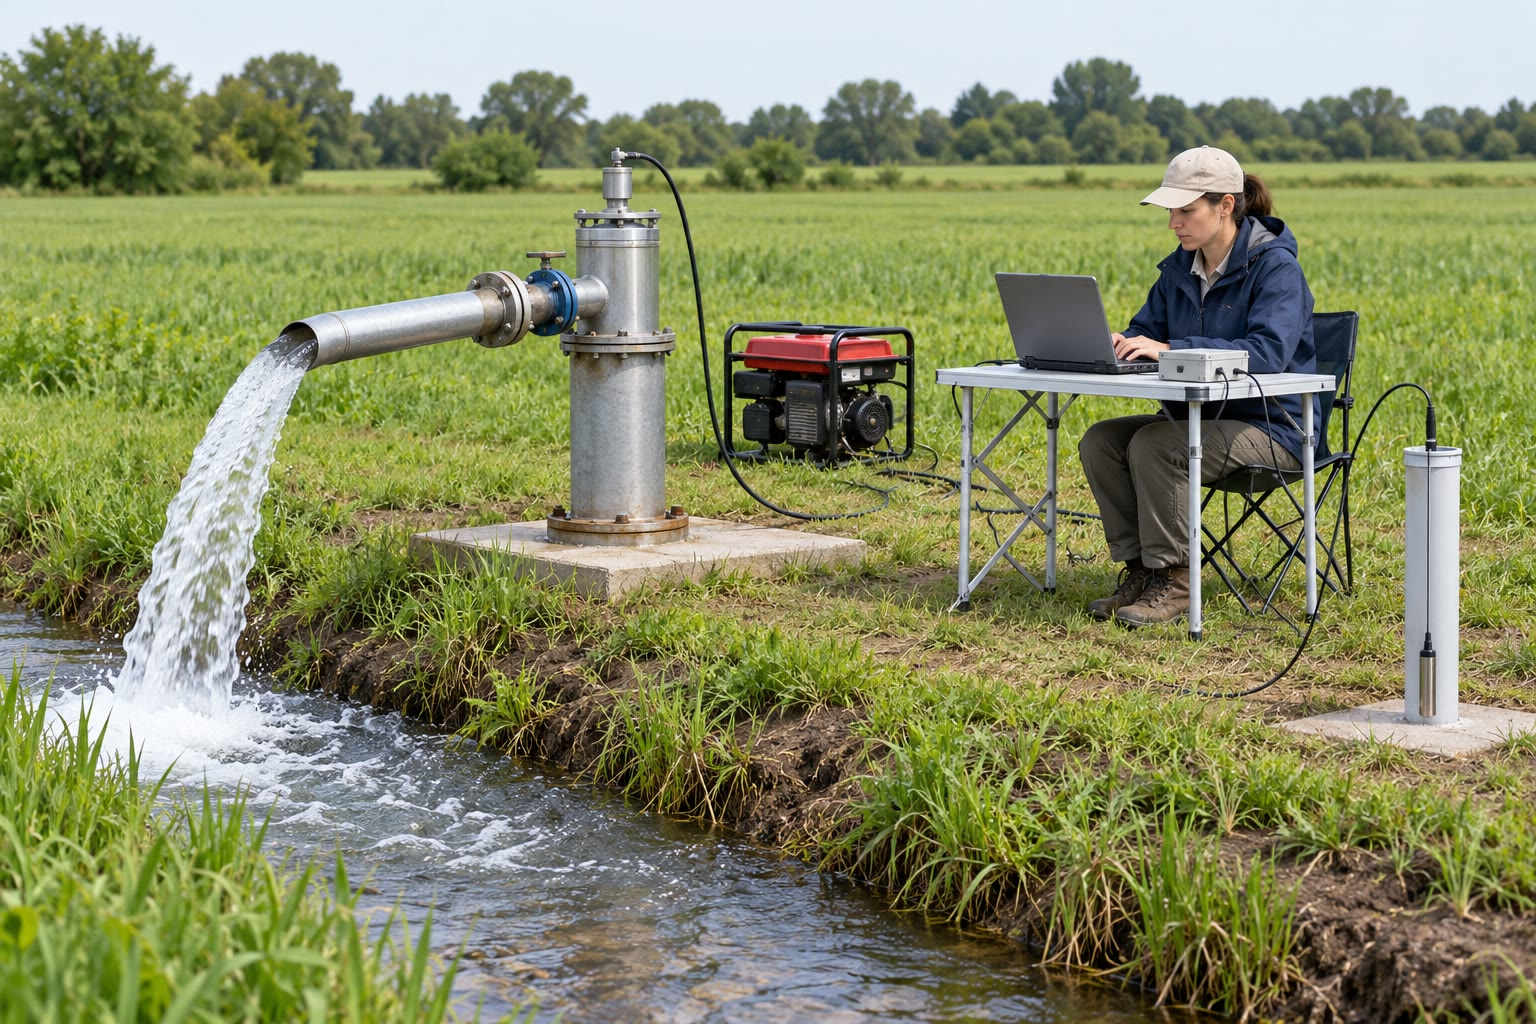
\includegraphics[width=\linewidth]{images/book5/ai/b3-pumping-test.jpg}

{\scriptsize पंपिंग परीक्षण: पंप किए जा रहे कुएँ का निकासी पाइप, एक जनित्र,
और एक भूजलवैज्ञानिक, जो लैपटॉप पर प्रेक्षण कुएँ का स्तर दर्ज कर रहा है
(AI से बनाया गया चित्रण)।}
\end{minipage}
\end{inthefield}
% ledger: heath:theis, heath:jacob, heath:water-levels, usgs:transducers

\section{विलेय परिवहन}\label{sec:b3:hydrogeology:transport}

भूजल में घुला विलेय जल के साथ \omterm{def:b3:hydrogeology:seepage}{रिसाव वेग} से वहन किया जाता है,
और चलते-चलते फैलता है: पड़ोसी रंध्रों का जल
भिन्न गति से और भिन्न पथों पर चलता है, और विलेय
भी विसरित होता है।

\begin{definition}[जलगतिक परिक्षेपण; परिक्षेपकता]\label{def:b3:hydrogeology:ade}
\emph{जलगतिक परिक्षेपण}\index{जलगतिक परिक्षेपण} वह है
बहते भूजल में विलेय का फैलाव, जो रंध्र-दर-रंध्र जल-वेग की विविधताओं से
और आणविक विसरण से होता है। प्रवाह के अनुदिश
इसे परिक्षेपण गुणांक $D = \alpha_Lv + D^*$ से वर्णित किया जाता है,
जहाँ $v$ \omterm{def:b3:hydrogeology:seepage}{रिसाव वेग} है, $D^*$ प्रभावी आणविक विसरणशीलता, और
$\alpha_L$, जो एक लंबाई है,
माध्यम की अनुदैर्घ्य \emph{परिक्षेपकता}\index{परिक्षेपकता} है।
\end{definition}

\begin{theorem}[अभिवहन-परिक्षेपण समीकरण]\label{thm:b3:hydrogeology:ade}
स्थिर \omterm{def:b3:hydrogeology:seepage}{रिसाव वेग} $v$ वाले एक-आयामी प्रवाह के अनुदिश,
अभिक्रिया न करने वाले विलेय की सांद्रता $C(x, t)$ समीकरण का पालन करती है:
\[
\frac{\partial C}{\partial t} = D\,\frac{\partial^2C}{\partial x^2} -
v\,\frac{\partial C}{\partial x} .
\]
यदि सांद्रता $C_0$ पर, $x = 0$ पर, $t = 0$ से स्थिर रखी जाती है, और माध्यम
आरंभ में विलेय से मुक्त है,
\[
\frac{C}{C_0} = \frac12\left[\operatorname{erfc}\frac{x - vt}{2\sqrt{Dt}} +
\mathrm e^{vx/D}\operatorname{erfc}\frac{x + vt}{2\sqrt{Dt}}\right] .
\]
\end{theorem}
\index{अभिवहन-परिक्षेपण समीकरण}

\begin{proof}
एकांक अनुप्रस्थ-काट और लंबाई $\mathrm dx$ के एक टुकड़े में, जिसकी प्रभावी
छिद्रता $n_e$ है, संचित विलेय $n_eC\,\mathrm dx$ है। इसका फ़्लक्स है
$n_e(vC - D\,\partial C/\partial x)$, जो जल के साथ वहन होता है और
परिक्षेपण द्वारा फैलता है, जैसे फ़िक का नियम विसरणशील पदार्थ को फैलाता है। संरक्षण से
$n_e\partial_tC = -\partial_x[n_e(vC - D\partial_xC)]$ प्राप्त होता है, यही समीकरण है।
यह कि सूत्र समीकरण को और शर्तों को संतुष्ट करता है, यहाँ स्वीकार किया जाता है;
इसके फैलाव की जाँच \cref{exo:b3:hydrogeology:12} में की गई है।
\end{proof}

जल के साथ चलते निर्देश-तंत्र में, $\xi = x - vt$, यह समीकरण
विसरण समीकरण बन जाता है, और अग्र भाग इस प्रकार फैलता है $\sqrt{2Dt} = \sqrt{2\alpha_L
vt} = \sqrt{2\alpha_Lx}$: अग्र भाग की चौड़ाई
तय की गई दूरी के वर्गमूल के अनुपात में बढ़ती है।

\begin{definition}[मंदन गुणक]\label{def:b3:hydrogeology:retardation}
जो विलेय संतुलन में और अपनी सांद्रता के अनुपात में कणों पर अधिशोषित होता है,
वह जल से धीमे चलता है। इसका
\emph{मंदन गुणक}\index{मंदन गुणक (सोखना)} होता है
\[
R = 1 + \frac{\rho_bK_d}{n} ,
\]
जहाँ $\rho_b$ माध्यम का शुष्क थोक घनत्व है, $n$ उसकी छिद्रता है और
$K_d$ वितरण गुणांक है, अर्थात ठोस के प्रति इकाई द्रव्यमान पर अधिशोषित द्रव्यमान
को जल में सांद्रता से भाग देने पर प्राप्त मान। विलेय $v/R$ वेग से चलता है
और $D/R$ के साथ परिक्षेपित होता है।
\end{definition}

\begin{omfigure}
\begin{tikzpicture}
\begin{groupplot}[group style={group size=2 by 1, horizontal sep=1.5cm},
  width=0.48\linewidth, height=0.4\linewidth,
  tick label style={font=\scriptsize}, label style={font=\small}, title style={font=\small}]
\nextgroupplot[xlabel={समय (दिन)}, ylabel={$C/C_0$ पर \qty{100}{m}},
  xmin=0, xmax=1000, ymin=0, ymax=1.05, title={प्रवेश वक्र},
  legend style={font=\scriptsize, at={(0.97,0.03)}, anchor=south east}]
% computed in figdata/bachelor-3/advection_dispersion.py
\addplot[omDef, thick] table[x=t, y=c1] {figdata/out/bachelor-3-advection_dispersion-btc.dat};
\addlegendentry{$\alpha_L = \qty{1}{m}$}
\addplot[omMeth, thick] table[x=t, y=c3] {figdata/out/bachelor-3-advection_dispersion-btc.dat};
\addlegendentry{$\alpha_L = \qty{3}{m}$}
\addplot[omThm, thick] table[x=t, y=c10] {figdata/out/bachelor-3-advection_dispersion-btc.dat};
\addlegendentry{$\alpha_L = \qty{10}{m}$}
\addplot[black, thick, densely dashed, forget plot] table[x=t, y=cR] {figdata/out/bachelor-3-advection_dispersion-btc.dat};
\node[font=\scriptsize, anchor=west, align=left] at (axis cs:640,0.45) {$\alpha_L = \qty{3}{m}$,\\ $R = 3$};
\addplot[black!40, densely dotted, forget plot] coordinates {(200,0) (200,1.05)};
\nextgroupplot[xlabel={दूरी (\unit{m})}, ylabel={$C/C_0$, 150 दिन बाद},
  xmin=0, xmax=160, ymin=0, ymax=1.05, title={प्रोफ़ाइल},
  legend style={font=\scriptsize, at={(0.03,0.03)}, anchor=south west}]
\addplot[omDef, thick] table[x=x, y=c1] {figdata/out/bachelor-3-advection_dispersion-profile.dat};
\addlegendentry{$\alpha_L = \qty{1}{m}$}
\addplot[omMeth, thick] table[x=x, y=c3] {figdata/out/bachelor-3-advection_dispersion-profile.dat};
\addlegendentry{$\alpha_L = \qty{3}{m}$}
\addplot[omThm, thick] table[x=x, y=c10] {figdata/out/bachelor-3-advection_dispersion-profile.dat};
\addlegendentry{$\alpha_L = \qty{10}{m}$}
\addplot[black!40, densely dotted, forget plot] coordinates {(75,0) (75,1.05)};
\end{groupplot}
\end{tikzpicture}

\par\smallskip{\small $x = 0$ पर निरंतर डाला गया एक विलेय, \omterm{def:b3:hydrogeology:seepage}{रिसाव वेग}
\qty{0.5}{m/d} वाले प्रवाह में। बाएँ पैनल में प्रवणता की दिशा में
\qty{100}{m} दूर पर समय के साथ सांद्रता: जल स्वयं
200 दिन बाद (बिंदीदार रेखा) पहुँचता है। \omterm{def:b3:hydrogeology:ade}{परिक्षेपकता} जितनी बड़ी हो, पहले संकेत उतने ही पहले
आते हैं और पूर्ण सांद्रता उतनी ही देर से। अधिशोषित विलेय, जिसका $R =
3$ है, तीन गुना देर से पहुँचता है। दाईं ओर, प्रवाह के साथ
150 दिन बाद सांद्रता, जब जल \qty{75}{m} चल चुका हो
(बिंदीदार रेखा)।}\label{fig:b3:hydrogeology:transport}
\end{omfigure}

परिक्षेपकताओं का मापन कठिन होता है, और व्यवहार में वे प्रायः
अंगूठे के नियमों से तय होती हैं। सबसे पुराना नियम अनुदैर्ध्य \omterm{def:b3:hydrogeology:ade}{परिक्षेपकता} को
प्लूम की लंबाई का दसवाँ भाग मानता है। क्षेत्र मापनों का एक संकलन, जो
1992 में प्रकाशित हुआ था, दिखाता है कि \omterm{def:b3:hydrogeology:ade}{परिक्षेपकता} प्रयोग के पैमाने के साथ बढ़ती है,
बड़े पैमानों पर विश्वसनीय मान कम हैं, और किसी एक पैमाने पर
मान दो या तीन परिमाण-कोटियों के परास में फैले होते हैं।
% ledger: epa:dispersivity

\section{अभ्यास}

\begin{exercise}[$\star$]\label{exo:b3:hydrogeology:1}
दो पीज़ोमीटर एक-दूसरे के बगल में भूमि पर लगे हैं, जो
संदर्भ-तल से \qty{120.0}{m} ऊपर हैं। पहले की छन्नी \qty{40}{m} गहराई पर है, और उसका जल
भूमि से \qty{12.5}{m} नीचे रहता है; दूसरे की छन्नी \qty{80}{m}
गहराई पर है, उसका जल भूमि से \qty{15.0}{m} नीचे है। उन्नयन
शीर्ष, दाब शीर्ष और \omterm{def:b3:hydrogeology:head}{जलीय शीर्ष} दोनों छन्नियों पर परिकलित कीजिए। जल उनके बीच किस
दिशा में बहता है, और किस ऊर्ध्वाधर प्रवणता के अंतर्गत?
\end{exercise}

\begin{exercise}[$\star$]\label{exo:b3:hydrogeology:2}
बालू का एक स्तंभ, जिसकी लंबाई \qty{50}{cm} और व्यास \qty{10}{cm} है, जिसका $K =
\qty{12}{m/d}$ और प्रभावी छिद्रता 0.35 है, \qty{30}{cm} के शीर्ष अंतर के अंतर्गत
जल प्रवाहित होता है। \omterm{def:b3:hydrogeology:darcy}{विशिष्ट विसर्जन}, लीटर प्रति
घंटे में प्रवाह और \omterm{def:b3:hydrogeology:seepage}{रिसाव वेग} परिकलित कीजिए।
\end{exercise}

\begin{exercise}[$\star$]\label{exo:b3:hydrogeology:3}
\qty{10}{\celsius} पर जल के लिए एक चूना-पत्थर का $K = \qty{2.5}{m/d}$ है
($\rho = \qty{999.7}{kg/m^3}$, $\mu = \qty{1.306e-3}{Pa.s}$)। इसकी \omterm{def:b3:hydrogeology:darcy}{आंतरिक पारगम्यता}
परिकलित कीजिए, और \qty{20}{\celsius} पर जल के लिए इसकी \omterm{def:b3:hydrogeology:darcy}{जलीय चालकता}
($\rho = \qty{998.2}{kg/m^3}$, $\mu =
\qty{1.002e-3}{Pa.s}$) ज्ञात कीजिए।
\end{exercise}
% ledger: nist:water

\begin{exercise}[$\star$]\label{exo:b3:hydrogeology:4}
वार्डन-3 का परिरुद्ध चूना-पत्थर \qty{180}{m} मोटा है, जिसका $K =
\qty{2.5}{m/d}$ है। इसकी \omterm{def:b3:hydrogeology:storage}{पारगमनता}, और वह \omterm{def:b3:hydrogeology:storage}{संचयिता} जो
होती यदि केवल जल का प्रसार, \num{9e-7} प्रति मीटर जलभृत प्रति मीटर शीर्ष पर,
जल मुक्त करता, परिकलित कीजिए। $S = \num{2e-4}$ से तुलना कीजिए।
\end{exercise}
% ledger: heath:storage

\begin{exercise}[$\star\star$]\label{exo:b3:hydrogeology:5}
\qty{1500}{m^3/d} पर लंबी अवधि तक पंपिंग के बाद अवनमन
बदलना बंद कर चुके हैं: पंप किए गए कुएँ से \qty{20}{m} दूर एक अवलोकन कुएँ में \qty{2.35}{m} और
\qty{200}{m} दूर वाले में \qty{0.82}{m}। जलभृत परिरुद्ध है और
\qty{40}{m} मोटा है। इसकी \omterm{def:b3:hydrogeology:storage}{पारगमनता} और \omterm{def:b3:hydrogeology:darcy}{जलीय
चालकता} परिकलित कीजिए।
\end{exercise}

\begin{exercise}[$\star\star$]\label{exo:b3:hydrogeology:6}
एक कुआँ \omterm{def:b3:hydrogeology:aquifer-types}{परिरुद्ध जलभृत} से \qty{1200}{m^3/d} पंप करता है, जिसका $T =
\qty{300}{m^2/d}$ और $S = \num{5e-4}$ है। $u$, $W(u)$ (श्रेणी से) और
\qty{300}{m} दूर का अवनमन, 1 दिन बाद और 10 दिन बाद, परिकलित कीजिए।
\end{exercise}

\begin{exercise}[$\star\star$]\label{exo:b3:hydrogeology:7}
वार्डन-3 परीक्षण के लिए ($T = \qty{450}{m^2/d}$, $S = \num{2e-4}$), कितने मिनट
बाद अवलोकन कुओं में कूपर--जैकब रेखा का उपयोग किया जा सकता है,
जो पंप किए गए कुएँ से \qty{60}{m} और \qty{500}{m} दूर हैं? इससे क्या संकेत मिलता है
कि छोटे परीक्षण के अवलोकन कुएँ कहाँ होने चाहिए?
\end{exercise}

\begin{exercise}[$\star\star$]\label{exo:b3:hydrogeology:8}
वार्डन चूना-पत्थर में एक-दूसरे से \qty{400}{m} दूर स्थित दो कुएँ प्रत्येक
\qty{2160}{m^3/d} पंप करते हैं। दोनों के बीच के मध्य-बिंदु पर 10 दिन बाद का अवनमन परिकलित कीजिए,
और दूसरे कुएँ के स्थान पर केवल पहले कुएँ के कारण अवनमन परिकलित कीजिए। प्रत्येक कुएँ का
पंपन दूसरे कुएँ को धन की हानि क्यों पहुँचाता है?
\end{exercise}

\begin{exercise}[$\star\star$]\label{exo:b3:hydrogeology:9}
बाँध के नीचे के \omterm{def:b3:hydrogeology:flow-net}{प्रवाह जाल} में प्रवाह वाहिकाएँ और शीर्ष-ह्रास गिनिए।
$K = \qty{5}{m/d}$ और $H = \qty{10}{m}$ लेकर, बाँध के प्रति
मीटर और \qty{300}{m} लंबे बाँध के नीचे का रिसाव परिकलित कीजिए।
\end{exercise}

\begin{exercise}[$\star\star\star$]\label{exo:b3:hydrogeology:10}
स्वच्छ बालू को \qty{50}{\micro\metre} त्रिज्या की सीधी नलिकाओं के रूप में,
0.30 छिद्रता के साथ प्रतिरूपित कीजिए। $k$ और $K$ परिकलित कीजिए (\qty{20}{\celsius} पर जल के लिए,
\cref{exo:b3:hydrogeology:3} देखिए),
और स्वच्छ बालू के परास से तुलना कीजिए। वास्तविक बालू की कौन-सी विशेषताएँ
प्रतिरूप में छूट जाती हैं, और उनमें से प्रत्येक $K$ को किस दिशा में बदलती है?
\end{exercise}
% ledger: nist:water, heath:k-chart

\begin{exercise}[$\star\star\star$]\label{exo:b3:hydrogeology:11}
(क)~दिखाइए कि कूपर--जैकब अवनमन $r_0 =
\sqrt{2.25\,Tt/S}$ पर शून्य हो जाता है। (ख)~परिरुद्ध वार्डन चूना-पत्थर में 30 दिन के पंपन के बाद $r_0$
परिकलित कीजिए, और उसी शैल के लिए अपरिरुद्ध अवस्था में, $S =
0.2$ लेकर। (ग)~\omterm{def:b3:hydrogeology:aquifer-types}{परिरुद्ध जलभृत} का शंकु उस सीमा तक क्यों पहुँच सकता है
जिसे देखना परीक्षण का उद्देश्य नहीं था?
\end{exercise}
% ledger: heath:jacob, heath:storage

\begin{exercise}[$\star\star\star$]\label{exo:b3:hydrogeology:12}
(क)~लंबी यात्रा दूरी के लिए $x$ पर भेदन वक्र समय में एक
समय में प्रसामान्य बंटन के निकट है, जिसका माध्य $x/v$ और मानक विचलन $\sigma_t
= \sqrt{2\alpha_Lx}/v$ है। अग्र भाग के प्रसार $\sqrt{2Dt}$ से इसे दिखाइए।
(ख)~\qty{100}{m} पर, $v = \qty{0.5}{m/d}$ के साथ, सांद्रता
\num{152.6}~दिन बाद \qty{16}{\percent} तक, और
\qty{84}{\percent} तक \num{247.2}~दिन बाद पहुँचती है। $\alpha_L$ का अनुमान लगाइए। (ग)~एक बलुई जलभृत में $\rho_b =
\qty{1.9}{g/cm^3}$ और $n = 0.30$ है; एक विलेय का $K_d =
\qty{0.32}{cm^3/g}$ है। $R$ परिकलित कीजिए।
\end{exercise}

\section{समस्या: वार्डन-3 पर पंपन परीक्षण}

\begin{problem}[{सप्ताहांत समस्या --- जलीय शीर्ष, एक पंपन परीक्षण और
परिरुद्ध वार्डन पहाड़ियों के चूना-पत्थर में एक प्रदूषक की यात्रा}]
\label{pb:b3:hydrogeology:1}
काल्पनिक कुआँ वार्डन-3 वार्डन पहाड़ियों के ग्रिड में (4500, 5000) पर खोदा गया है,
भू-ऊँचाई \qty{363.2}{m} से शुरू होकर, जुरासिक शेल के आर-पार
जुरासिक चूना-पत्थर तक जाता है, जिसका ऊपरी सिरा
\qty{282.5}{m} और आधार \qty{102.5}{m} पर है (दोनों समुद्र-तल से ऊपर); कुआँ चूना-पत्थर की
पूरी मोटाई पर खुला है। परीक्षण से पहले इसमें जल
भू-सतह से \qty{45.0}{m} नीचे था।

\medskip\noindent\textbf{भाग I --- जलभृत और उसका प्राकृतिक प्रवाह।}
\begin{enumerate}
\item कुएँ पर शेल और चूना-पत्थर की मोटाई परिकलित कीजिए।
\item चूना-पत्थर में शीर्ष और उसके ऊपरी सिरे पर दाब-शीर्ष परिकलित कीजिए।
  यहाँ चूना-पत्थर \omterm{def:b3:hydrogeology:aquifer-types}{परिरुद्ध जलभृत} क्यों है?
\item चूना-पत्थर से खुले तीन पीज़ोमीटर P1 (4300, 5250), P2
  (4850, 5150) और P3 (4550, 4650) पर स्थित हैं, जिनके शीर्ष 318.96, 317.34 और
  \qty{317.52}{m} हैं। $h = ax + by + c$ लिखकर $a$ और $b$ ज्ञात कीजिए।
\item \omterm{def:b3:hydrogeology:head}{जलीय प्रवणता} और वह दिगंश परिकलित कीजिए, जिस ओर
  जल बहता है।
\end{enumerate}

\medskip\noindent\textbf{भाग II --- पंपन परीक्षण।} कुएँ को दो दिन तक
\qty{2160}{m^3/d} की दर से पंप किया जाता है। \qty{60}{m} दूर एक अवलोकन कुएँ में
अवनमन इस प्रकार हैं:
\begin{center}
\begin{tabular}{l*{11}{c}}
\hline
$t$ (\unit{min}) & 1 & 2 & 3 & 5 & 7 & 10 & 15 & 20 & 30 & 45 & 60\\
$s$ (\unit{m}) & 0.18 & 0.36 & 0.48 & 0.64 & 0.77 & 0.88 & 1.04 & 1.15 & 1.30 & 1.45 & 1.56\\
\hline
$t$ (\unit{min}) & 90 & 120 & 180 & 240 & 360 & 480 & 720 & 960 & 1440 & 2160 & 2880\\
$s$ (\unit{m}) & 1.71 & 1.82 & 1.98 & 2.08 & 2.24 & 2.35 & 2.50 & 2.61 & 2.77 & 2.92 & 3.03\\
\hline
\end{tabular}
\end{center}
\begin{enumerate}[resume]
\item $s$ को $\log_{10}t$ के विरुद्ध आलेखित कीजिए। कौन-से आरंभिक बिंदु सीधी
  रेखा से हटते हैं, और क्यों?
\item सीधे भाग से प्रति लघुगणक चक्र अवनमन मापिए।
\item \omterm{def:b3:hydrogeology:storage}{पारगमनता} परिकलित कीजिए।
\item वह समय $t_0$ ज्ञात कीजिए जिस पर रेखा शून्य अवनमन को काटती है।
\item \omterm{def:b3:hydrogeology:storage}{संचयिता} परिकलित कीजिए।
\item जाँच कीजिए कि प्रयुक्त बिंदुओं के लिए $u \le 0.05$ है।
\item चूना-पत्थर की \omterm{def:b3:hydrogeology:darcy}{जलीय चालकता} परिकलित कीजिए।
\end{enumerate}

\medskip\noindent\textbf{भाग III --- अवनमन शंकु।} यहाँ से $T =
\qty{450}{m^2/d}$ और $S = \num{2e-4}$ लीजिए।
\begin{enumerate}[resume]
\item अवलोकन कुएँ में 2 दिन बाद थीस अवनमन परिकलित कीजिए और
  उसकी तुलना अभिलेख से कीजिए।
\item \qty{1}{km} दूर एक खेत का कुआँ उसी चूना-पत्थर से जल लेता है। इसका
  अवनमन 30 दिन के पंपन के बाद परिकलित कीजिए।
\item 30 दिन बाद जैकब की दूरी $r_0$ परिकलित कीजिए। यह जलभृत के किनारों
  और वार्डन पहाड़ियों के भ्रंश के बारे में क्या बताती है?
\item 30 दिनों में पंप किया गया आयतन परिकलित कीजिए। \omterm{def:b3:hydrogeology:aquifer-types}{परिरुद्ध जलभृत} में
  यह आयतन कहाँ से आता है?
\item $S = 0.18$ लेकर, यदि चूना-पत्थर अपरिरुद्ध होता, तो खेत पर अवनमन की
  तुलना कैसी होती?
\end{enumerate}

\medskip\noindent\textbf{भाग IV --- एक प्रदूषक।} एक घुले हुए प्रदूषक का रिसाव
कुएँ से \qty{200}{m} दूर चूना-पत्थर तक पहुँचता है।
प्रभावी छिद्रता 0.18 और \omterm{def:b3:hydrogeology:retardation}{मंदन गुणक} 2.5 लीजिए।
\begin{enumerate}[resume]
\item पंपन से पहले, भाग~I के प्राकृतिक प्रवाह का \omterm{def:b3:hydrogeology:darcy}{विशिष्ट विसर्जन} और \omterm{def:b3:hydrogeology:seepage}{रिसाव
  वेग} परिकलित कीजिए।
\item जल को \qty{200}{m} तय करने में और प्रदूषक को
  कितना समय लगेगा?
\item कुएँ के पंपन होने पर और उसके ऊपर-प्रवणता में स्थित रिसाव के साथ, प्रवाह
  कुएँ की ओर त्रिज्यीय हो जाता है। दिखाइए कि जल को $t = \pi n_e b
  r^2/Q$ समय लगता है, दूरी $r$ से कुएँ तक पहुँचने में, प्राकृतिक प्रवाह की
  उपेक्षा करते हुए, और उसे जल तथा प्रदूषक के लिए परिकलित कीजिए।
\item दूरी के दसवें भाग के बराबर \omterm{def:b3:hydrogeology:ade}{परिक्षेपकता} के अनुभवजन्य नियम से,
  कुएँ पर अग्र भाग के प्रसार $\sqrt{2\alpha_Lx}$ का अनुमान लगाइए। प्रथम आगमन के लिए
  इसका क्या अर्थ है?
\item क्या पंपन जारी रहना चाहिए? एक पक्ष में और एक विपक्ष में तर्क दीजिए।
\item वार्डन चूना-पत्थर जलभृत की \omterm{def:b3:hydrogeology:storage}{पारगमनता} वर्ग मीटर प्रति दिन में,
  दो सार्थक अंकों तक दीजिए।
\end{enumerate}
\end{problem}
% ledger: heath:jacob, heath:theis, heath:storage, epa:dispersivity, region:name
